\documentclass{standalone}

\begin{document}

\section[CHIMeRA analyses]{CHIMeRA analyses}\label{chimera:res}

The large amount of informations provided by the \textsf{CHIMeRA} network has to be analyzed to prove its efficiency.
A preliminary analysis was performed evaluating the node degree centrality.
The degree centrality is the simpler measure to quantify the importance of a node inside a network and since our network-of-networks structure includes multiple node types we monitored it for each of them\footnote{
  We chose the degree centrality rather than other standard measures due to its numerical-simplicity/informative ratio.
  The \textsf{CHIMeRA} network includes a large amount of nodes so the algorithm complexity drastically affect the time performances.
  The degree centrality is given by the simple sum of the in- out-connections and thus it is faster also with large matrix as in our case.
}.
First of all we evaluated the number of connections of each node unpacking the value according to the possible node types.
In this way we can perform a preliminary overview of the full set informations in the network.
The summary results obtained by the degree centrality are shown in Tab.~\ref{tab:chimera_degree}.

\begin{table}
\centering
\begin{tabular}{lccccccccccccccc}
\hline \rowcolor{darkgrayrow}
       & global  & disease &   drug & food & gene & metabolite & phenotype &  SNP & metabolic & disease   & drug-action & drug-metabolism &  signaling       & physiological   & macro   \\
\rowcolor{darkgrayrow}
       & degree  &         &        &      &      &            &           &      & pathway   & pathway   & pathway     &  pathway        &  pathway         &  pathway        & pathway \\
mean   &  121.44 &   18.54 &  93.59 & 0.03 & 1.96 &       0.37 &      5.50 & 0.65 &      0.09 &      0.05 &        0.14 & $6\times10^{-3}$& $4\times10^{-3}$ &$1\times10^{-3}$ &   0.48  \\
std    &  784.86 &  109.25 & 737.60 & 0.32 &38.81 &     154.73 &    100.09 &21.96 &      2.81 &      1.27 &        6.79 &            0.28 &             0.29 &            0.07 & 106.06  \\
min    &       1 &       0 &      0 &    0 &    0 &          0 &         0 &    0 &         0 &         0 &           0 &               0 &                0 &               0 &      0  \\
25\%   &       1 &       0 &      0 &    0 &    0 &          0 &         0 &    0 &         0 &         0 &           0 &               0 &                0 &               0 &      0  \\
50\%   &       2 &       1 &      0 &    0 &    0 &          0 &         0 &    0 &         0 &         0 &           0 &               0 &                0 &               0 &      0  \\
75\%   &       7 &       3 &      0 &    0 &    0 &          0 &         0 &    0 &         0 &         0 &           0 &               0 &                0 &               0 &      1  \\
max    &  108147 &   22911 &  17750 &   12 & 5605 &      85236 &      9732 & 4866 &       594 &       283 &        1006 &              60 &               49 &              13 &  59993  \\
\hline\\
\end{tabular}
\caption{
}
\label{tab:chimera_degree}
\end{table}

For each node type we computed the average number of connections and the main important parameters of each distribution (minimum, maximum, standard deviations and percentiles).
These preliminary results confirm the previous discussion about the network matrix structure: the only node type which has at least one connection is only the disease one (ref. min row in Tab~\ref{tab:chimera_degree}).
A better visualization of the network structure could be done counting the average number of connections between each group of nodes, i.e the block matrix visualization of the underlying bipartite-graphs.
In Fig.~\ref{fig:chimera_bipartite} is shown the block matrix representation.

\begin{figure}[htbp]
\centering
\def\svgwidth{\textwidth}
\input{./img/chimera_net_mat.pdf_tex}
\caption{Block matrix representation of the \textsf{CHIMeRA} network.
We computed the average number of connections between each node group and the bipartite-graphs structure is highlight.
}
\label{fig:chimera_bipartite}
\end{figure}

In Fig.~\ref{fig:chimera_bipartite} we can better appreciate the connections between the available informations and moreover we can visualize and quantify them.
As expected the only node type which is connected to all the others is the \emph{disease} one: the only exception is given by \emph{food} nodes which are not directly connected with the diseases since their informations are available only in the DrugBank database and thus their connections are related only with \emph{drug} nodes.
Our network-of-networks structure is very sparse and we have not direct informations of the major part of combinations (null blocks).
The only two node types which show a reasonably good interactions with the other blocks are the \emph{disease} and \emph{drug} ones\footnote{
  For sake of clarity we have to highlight also the two diagonal blocks in our matrix given by these two node types.
  They arise from the synonyms and related causes in the first case (informations provided by the synonym dictionaries and from the RXList database), while in the second case they highlight the synergies or not (informations given by the DrugBank database).
  A network adjacency matrix tends to nullify the diagonal informations and node self-loops to prevent numerical issues and moreover to increase the amount of mathematical theorems for its analysis.
  We would stress that the showed matrix is not the adjacency matrix of the \textsf{CHIMeRA} network but it is an aggregate representation of it.
  Thus in our network each node has connections only with other nodes and no self-loops are present.
}.

The sparsity of \textsf{CHIMeRA} network highlight all the pros and cons of our work.
More a matrix is sparse and more its management could be efficient from a numerical point-of-view: we are able to use a wide range of algorithms developed and tuned for the sparse algebra and also the memory occupation could be optimized that is a crucial task when we work with such a big quantity of data.
At the same time it also highlights the potentiality of our work: each block connection derives from a single database evaluation and we can reasonably assume that each block represents a possible output of query performed on that database.
In our global database we have the join merging of all these informations and using at least the 2-order connections (the nearest neighbors of each nearest neighbor of a node) we could obtain a mapping of all the available informations for each node.
Moving along the matrix blocks, in fact, we can start from a gene an we can only see the associated disease informations which is comparable to a single-database query; since each disease is connected to all the other node types, the 2-order connections give us a panoramic view of all the biological compounds associated to that gene.
This process is equivalent to an inference procedure of the missing blocks: if a gene is connected only to disease types since all the other blocks are null we could infer the missing blocks using the links provided by the disease nodes.
This is the real power of such a network-of-networks structure.
We would stress that the inference procedure could bring to incorrect biological associations since it represents only an hypothesis unbacked up by data.
However, using more databases source we can easily integrate the missing informations using the developed processing pipeline and thus increase the reliability of our hypothesis.

To further investigate the informations provided by our network using the computed degree scores, we evaluated the degree distributions of node types.
In Fig.~\ref{fig:chimera_degree} we show the degree distributions obtained considering different node type individually.

\begin{figure}[htbp]
\centering
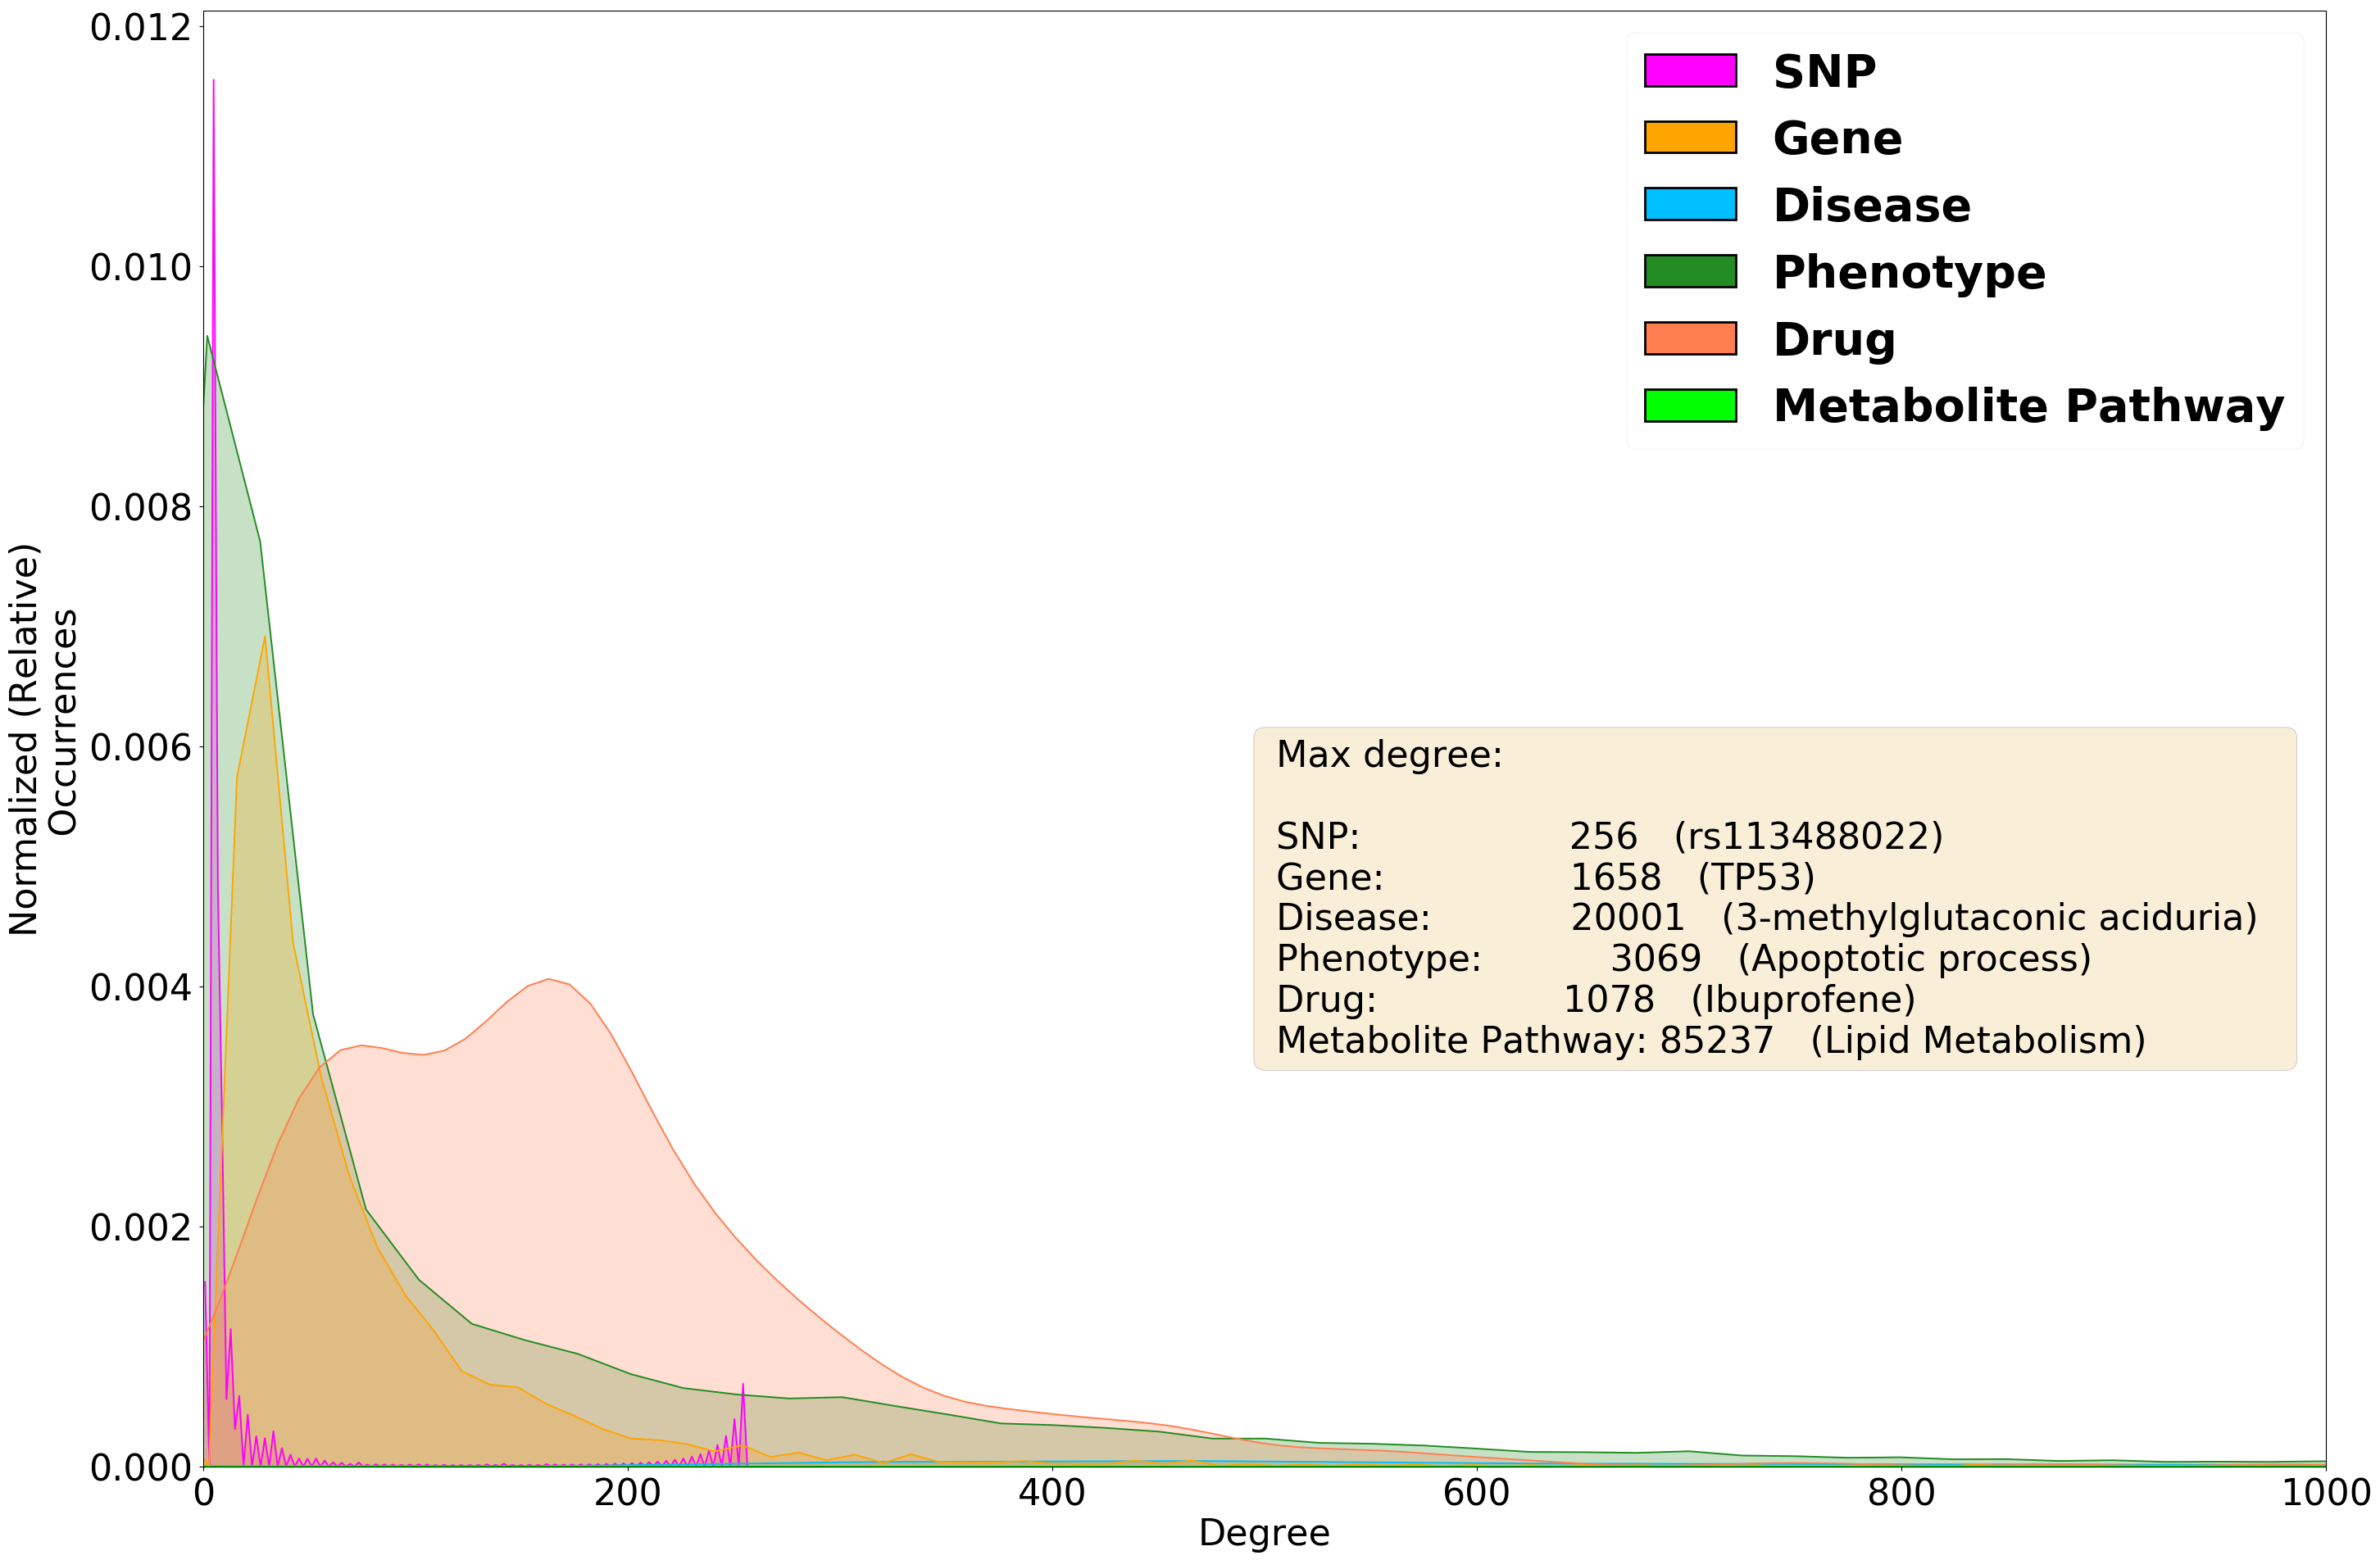
\includegraphics[width=.8\linewidth]{degree.png}
\caption{CHIMeRA degree distributions for different node types.
The plot is cut for visualization purposes.
The maximum degree node informations are highlight in the box.
}
\label{fig:chimera_degree}
\end{figure}

All the distributions showed in Fig.~\ref{fig:chimera_degree} have long tails but we cut them for visualization purposes.
As expected and already highlighted by the previous analyses, the major part of node types have a not negligible amount of nodes with very low connectivity.
Many node types have also isolated elements, i.e nodes with 0 connectivity.
This behavior could be due to two possible causes: 1) our pipeline tends to remove some informations and thus some true positive associations; 2) there are some missing informations in the original databases that could not be overcome by our merging.
Since the most part of isolated nodes are given by \emph{metabolites} (ref. Fig.~\ref{fig:chimera} in which the green dots around the plot are isolated metabolite nodes) we checked into the HMDB database the origin of this issues.
In a not negligible number of cases the HMDB does not provide a disease association to a given metabolite and this proves our second hypothesis, preserving the efficiency of our pipeline.

A more interesting result is obtained considering the most central nodes, i.e the node related to the maximum degree score.
This information could be used also as validity check of the structured.
As in the \textsf{SymptomsNet} case (ref. \ref{chimera:symptomsnet}), we expect a reasonable interpretation of the most central nodes.
These results are showed in the yellow box in Fig.~\ref{fig:chimera_degree}.

The most central node for the SNP node type is the \href{https://www.ncbi.nlm.nih.gov/snp/rs113488022}{\textsf{rs113488022}}, well known gene-mutation validated by 72 public research.
This SNP is related to a wide range of cancer diseases and its clinical significance has been proved in different studies.
It is always hard to discuss about the more or less importance of a SNP mutation compared to the others, but its relation to many disease types confirm its centrality score in our network structure.
A more easy interpretable results is given by the most central gene, the \href{https://ghr.nlm.nih.gov/gene/TP53}{\textsf{TP53}}.
The \textsf{TP53} is a crucial gene in many tumor diseases and its importance is well mirrored in our network structure.
The major part of diseases inserted into public databases are related to tumor researches and thus it was quite obvious to obtain a most centrality of this gene in our network.
For the same reasons also the most central node for the \emph{phenotype} type should be a tumor related characteristics: as expected the most central node in this case is given by the \textsf{apoptotic process}, i.e the process which regulates the programmed cell death, which is largely involved in tumor diseases.

As previously discussed for the \emph{disease} and \emph{drug} types we have to consider the large set of available connections thus we could expect that a central node in these cases would be given by a quite generic entry.
For the \emph{disease} type, in fact, we found as most central node the \href{https://en.wikipedia.org/wiki/3-Methylglutaconic_aciduria}{\textsf{3-methylglutaconic aciduria}}, a congenital metabolism anomaly related to leukemia.
Despite this disease could be considered quite rare its importance in our network structure is certainly given by the large amount of metabolite connections (we remember that the HMDB database provide a very large amount of \emph{metabolite} nodes that overcome the number of all the other node types, except by the SNPs).
The large quantity of metabolites in our structure certainly weight on the number of disease connections, thus we found as more central a metabolic disease than a genetic one.
Moreover, we have also to take into account that this disease is also related to the leukemia disease, so we would have also a large set of genes and SNPs associated to it.

Considering the \emph{drug} type we obtained a very common drug as expected, given by the \emph{Ibuprofene}.
The \emph{Ibuprofene}, in fact, could be used for a wide range of diseases and it is reasonable to assume that its number of connections is greater than other (more selective) drugs.

A key note has to be spent for the \emph{metabolite pathway} type in which there are not apparently reasonable explanations which prefer the found \textsf{lipid metabolism} to other macro-metabolite pathways.
To explain its centrality we once more time come back to the original databases and to the HMDB in this case.
By a deeply inspect of the metabolite databases we noticed that the major part of them are studied using NMR chemical shift procedure.
The NMR chemical shift is a very common spectroscopy procedure to analyze biological compounds but its signal is hardly related to particular nucleus types (e.g $^1H$, $^{13}C$, $^{15}N$).
We could broadly describe this technique saying that as much hydrogen-like or carbonic-like structures are found into the biological sample and much the signal should be easy to analyze.
The metabolite relation to the lipid metabolism is thus easy to study than other metabolism kinds due to the large quantity of resonant nuclei involved.
This proved the most centrality of the \textsf{lipid metabolism} regard other metabolite pathways.

These results are only preliminary analyses of the \textsf{CHIMeRA} network but they are already able to clarify some potentiality usage of our network-of-networks approach.
The only thing that remain to discuss is about the usability and release of this database to the research community.


\end{document}
